% id: 0198
% book: RPM 중3-2 수학 · 02 삼각비의 활용
% section: 유형 07 삼각형의 높이 구하기 – 주어진 각 중 한 각이 둔각인 경우
% figure: crop:fig-0198.png
% answer: ①
% answer_source: 답지
% variant_level: 0 (원본 전사)
% 이 파일은 build.mjs 가 items.json 에서 만든다. 고칠 때는 items.json 을 고친다.
\noindent\begin{minipage}[t]{0.58\linewidth}\vspace{0pt}\raggedright 오른쪽 그림과 같이 $\triangle\pt{ABC}$의 꼭짓점~$\pt{A}$에서 $\seg{BC}$의 연장선에 내린 수선의 발을 $\pt{H}$라 할 때, 다음 중 $\seg{AH}$의 길이를 구하는 식은?\end{minipage}\hfill\begin{minipage}[t]{0.4\linewidth}\vspace{0pt}\centering \setlength{\dmfigw}{88.2pt}\ifdim\dmfigw>\linewidth\setlength{\dmfigw}{\linewidth}\fi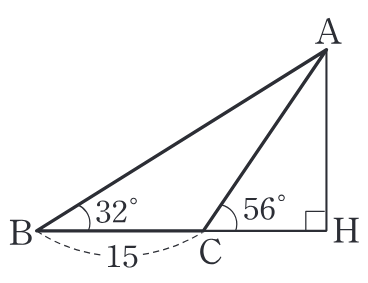
\includegraphics[width=\dmfigw]{figures/fig-0198.png}\end{minipage}\par
\begin{choicesii}{\rule[-3ex]{0pt}{8ex}$\dfrac{15}{\tan 58^\circ-\tan 34^\circ}$}{\rule[-3ex]{0pt}{8ex}$\dfrac{15}{\tan 58^\circ+\tan 34^\circ}$}{\rule[-3ex]{0pt}{8ex}$\dfrac{15}{\tan 56^\circ-\tan 32^\circ}$}{\rule[-3ex]{0pt}{8ex}$\dfrac{15}{\tan 56^\circ+\tan 32^\circ}$}{\rule[-3ex]{0pt}{8ex}$15(\tan 56^\circ-\tan 32^\circ)$}\end{choicesii}
